%!TEX root = ../thesis_a4.tex

\chapter{Applications}
\label{chap:applicatoins}

\section{Introduction}
\label{sec:applications_introduction}

The research work presented in this thesis has several applications. A number of these applications are already described in~\secref{sec:motivation}. While some applications such as \gls{raga}-based music retrieval and music discovery are relevant mainly in the context of large audio collections, there are several applications that can be developed on the scale of the music collection compiled in the CompMusic project. In this chapter, we present some concrete examples of such applications that have already incorporated parts of our work presented in this thesis. We provide a brief overview of Dunya, a collection of music corpora and software tools developed during the CompMusic project (\chapref{chap:corpus_music_corpora_and_datasets}) and, \Gls{saraga} and \Gls{riyaz}, the mobile applications developed within the technology transfer project, \gls{camut}. In addition, we present three web demos that showcase parts of the outcomes of our computational methods. We also briefly present one of our recent studies that perform musicologically motivated exploration of melodic structures in \gls{iam}. It serves as an example of how our methods can facilitate investigations in computational musicology.

\section{Dunya}
\label{sec:applications_dunya}

Dunya\footnote{\url{http://dunya.compmusic.upf.edu/}} comprises the music corpora and the software tools that have been developed as part of the CompMusic project. It includes data for five music traditions - Hindustani, Carnatic, Turkish Makam, Jingju and Andalusian music. By providing access to the gathered data (such as audio recordings and metadata), and the generated data (such as audio descriptors) in the project, Dunya aims to facilitate study and exploration of relevant musical aspects of different music repertoires. CompMusic corpora mainly comprise audio recordings and complementary information that describes those recordings. This complementary information can be in the form of the relevant metadata, and melody, rhythm, and structural descriptors that are computationally extracted from the audio recordings. The metadata for each recording is aggregated from multiple data sources: MusicBrainz, for the editorial metadata and, Wikipedia, for artists' biographies\footnote{An~example~of~a~biography,~\url{https://en.wikipedia.org/wiki/T._M._Krishna}} and related information. For a detailed description of Dunya we refer to~\cite{dunya_porter}.

To extract the music descriptors mentioned above Dunya uses \gls{essentia} and a set of software packages developed for specific music traditions. Our work on tonic identification is already integrated in to \gls{essentia}, and thus, is available in Dunya. The implementation of our other methods for pattern discovery and \gls{raga} recognition will also be integrated into \gls{essentia}. 

There are two modes in which Dunya provides access to the data mentioned above: a web-based interface, and a \acrshort{rest} \acrshort{api}. The web-based GUI\footnote{\url{http://dunya.compmusic.upf.edu/}} is mainly meant to browse through the music corpora, listen to the music recordings, and visualize the extracted music descriptors that are time-synchronized with the music. In a way, it provides a medium for enhanced music listening. In addition, for every recording the associated metadata is also shown, which provides the surrounding context to better appreciate the music performance. A screenshot of the recording page for a music piece\footnote{\url{http://dunya.compmusic.upf.edu/hindustani/recording/72df913b-ac52-4798-990d-72e04a64bd8c/raga-ragesri}}\footnote{\url{http://musicbrainz.org/recording/72df913b-ac52-4798-990d-72e04a64bd8c}} in Hindustani music is shown in~\figref{fig:dunya_recording}. We see that there are three main panes, the metadata pane towards top-left, rhythm pane at the top and melody pane at the bottom. The metadata pane displays the editorial and the automatically generated metadata. In this pane, the main description of the melodic aspects of a performance is given by its tonic and the \gls{raga} label, indicated by the arrows numbered 1~and~5, respectively. The melody pane at the bottom displays a coarse timbral representation on top which the predominant pitch contour is shown (indicated by arrow-3). In the same pane, the solid horizontal line (indicated by arrow-2) marks the tonic frequency of the recording. This frequency corresponds to the base \gls{svara} Sa in the performance, and it acts as a reference to better interpret the frequency intervals in the continuous pitch contour. The second octave of the tonic frequency is also indicated by a dashed horizontal line. Along with the predominant pitch contour its histogram is also shown (arrow-4), which summarizes the pitch content in the entire performance. 

\begin{sidewaysfigure}
	\begin{center}
		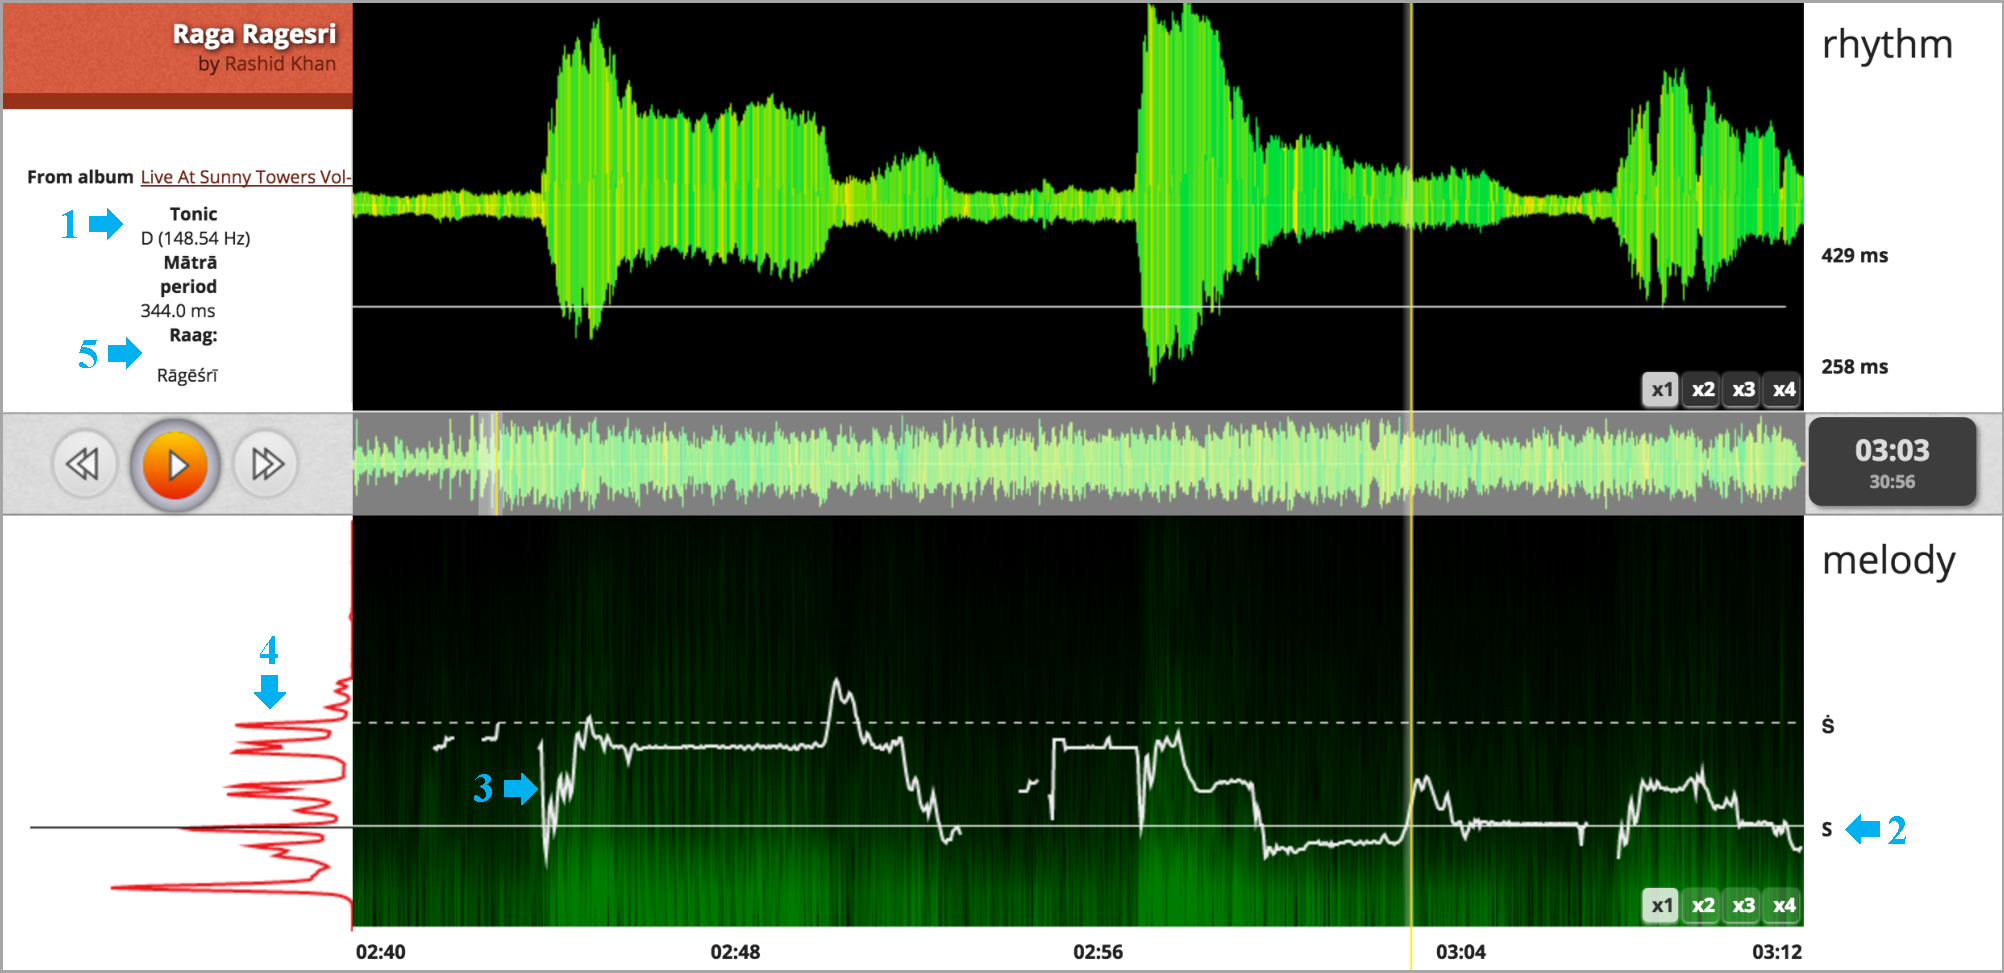
\includegraphics[width=\figSizeHundred]{ch08_applications/figures/dunyaScreenshot.pdf}
		\end{center}
		\caption[Screenshot of the recording page in Dunya]{Screenshot of the recording page in Dunya showing extracted music descriptors and associated metadata.}
		\label{fig:dunya_recording}
\end{sidewaysfigure}

While the web interface provides an easy and a quick access to the data, for a more comprehensive access mainly meant for researchers and developers, Dunya provides a \acrshort{rest} \acrshort{api}. Through the \acrshort{api} it exposes audio recordings, gathered metadata and extracted music descriptors. It can be used to access the existing datasets, as well as to create new datasets using the CompMusic corpora. To further facilitate the usage of this \acrshort{api}, a Python\footnote{\url{https://www.python.org/}} package, \gls{pycompmusic}\footnote{\url{https://github.com/MTG/pycompmusic}}, is provided. Using this tool, with just a few lines of code, the entire corpora and associated metadata can be retrieved. An example usage of \gls{pycompmusic} is shown below.

%\lstset{language=Python,
%	numbers=left,                    % where to put the line-numbers; possible values are (none, left, right)
%	numbersep=5pt,
%	basicstyle=\footnotesize,
%	numberstyle=\tiny,
%	frame=tb,
%	columns=fullflexible,
%	showstringspaces=false
%	}
%
%\begin{lstlisting}[frame=bt] 
%from compmusic import dunya as dn
%from compmusic.dunya import carnatic as ca										
%
%dn.set_token("60312f59428916bb854adaa208f55eb35c3f2f07")		#authorization
%
%recs = ca.get_concerts()																	  #Fetching all the concerts
%
%len(recs)
%
%\end{lstlisting}
{
	\small
\begin{verbatim}
In [1]: from compmusic import dunya as dn
In [2]: from compmusic.dunya import carnatic as ca
In [3]: dn.set_token("<dunya api token>")
In [4]: concerts = ca.get_concerts()
In [5]: len(concerts)
Out[5]: 328
In [6]: concerts[1]
Out[6]: 
       {u'mbid': u'c5d9d3bd-bc01-4104-b874-d55219bd0e54',
        u'title': u'Madrasil Margazhi 2006'}
In [7]: recs = ca.get_recordings()
In [8]: len(recs)
Out[8]: 3533
In [9]: recs[1]
Out[9]: 
       {u'mbid': u'01f863b7-46b4-44f5-b547-fcbaa1f66348',
        u'title': u'Vetta Veli'}        
\end{verbatim}
}

This is an example of querying the metadata for the Carnatic music collection\footnote{\url{https://musicbrainz.org/collection/55412ad8-1b15-44d5-8dc8-9c3cb0cf9e5d}} in the CompMusic corpora. The first step is to import the relevant modules provided in the PyCompMusic package (ln~[1] and [2]), followed by a user authentication, which requires a Dunya \acrshort{api} token (ln~[3]). This token can be obtained by registering in to Dunya. We then query for a list of all 328 concerts in the Carnatic music collection (ln~[4]), and the information about each concert is returned in a dictionary (Out~[6]). Subsequently, we also present a query to obtain a list of all 3533 recordings in the collection (ln~[7]), and show the structure of the response (Out~[9]). Using the \acrshortpl{mbid} of the concerts and the recordings we can obtain more information about those entities. The Dunya \acrshort{api} provides access to the editorial metadata, the audio recordings, and the extracted audio features for all the music collections in the CompMusic corpora.

\section{Mobile Applications: \glsentrytext{saraga} and \glsentrytext{riyaz}}
\label{sec:mobile_apps_camut}

\gls{saraga} and \gls{riyaz} are two mobile applications developed as a part of the \gls{camut}\footnote{\url{http://mtg.upf.edu/projects/camut}} project, which aims to explore the commercial exploitation of the technologies developed in the CompMusic project. These applications aim to foster learning, teaching and appreciation of Indian music forms. Both these applications incorporate parts of the outcome of our research work presented in this thesis. We provide below a brief description of these applications. 

\subsubsection{\glsentrytext{saraga}}
\label{sec:saraga}

\Gls{saraga} is a mobile application that provides an enriched listening atmosphere over a collection of Carnatic and Hindustani music that is released under the Creative Commons license\footnote{\url{https://creativecommons.org/}}. It is meant for music connoisseurs and students of these art music traditions to navigate, discover and listen to the music using culturally relevant concepts. \gls{saraga} contains inclusive designing of innovative visualizations and inter and intra-song navigation interfaces that present musically rich information to the user in a compact way. The time synchronized visualizations of musically relevant facets such as melodic patterns, \gls{sama} locations and sections provide a user with better understanding and appreciation of these music traditions.

\begin{figure}
	\centering
	\begin{subfigure}[b]{0.48\textwidth}
		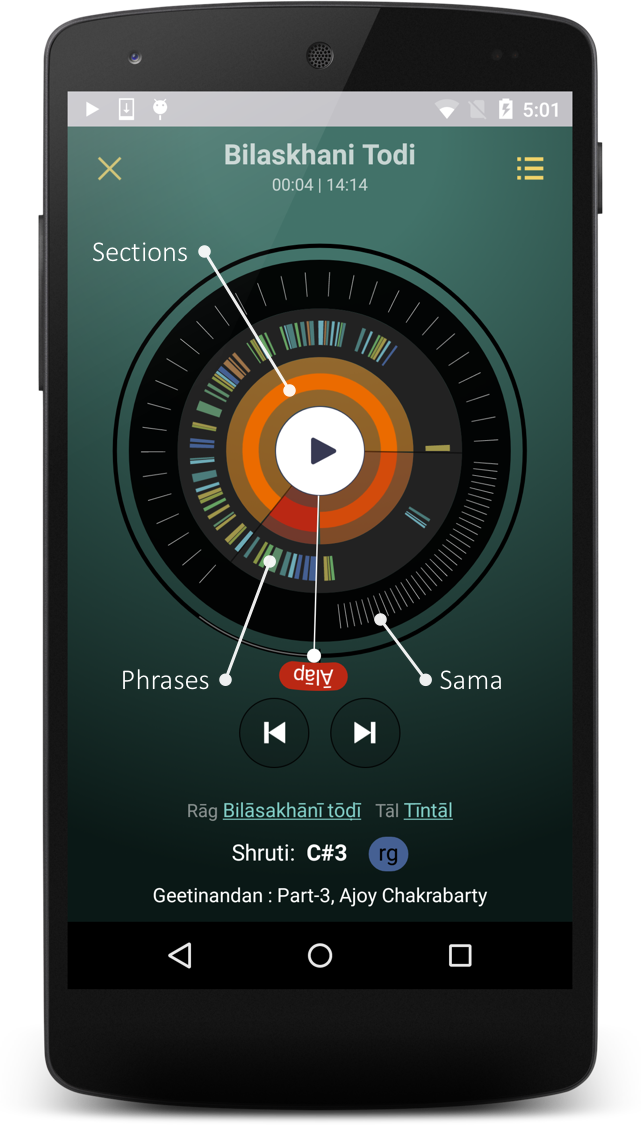
\includegraphics[width=\figSizeNinety]{ch08_applications/figures/saraga1.png}
		\caption{Full music piece}
		\label{fig:saraga_full_piece}
	\end{subfigure}
	\begin{subfigure}[b]{0.48\textwidth}
		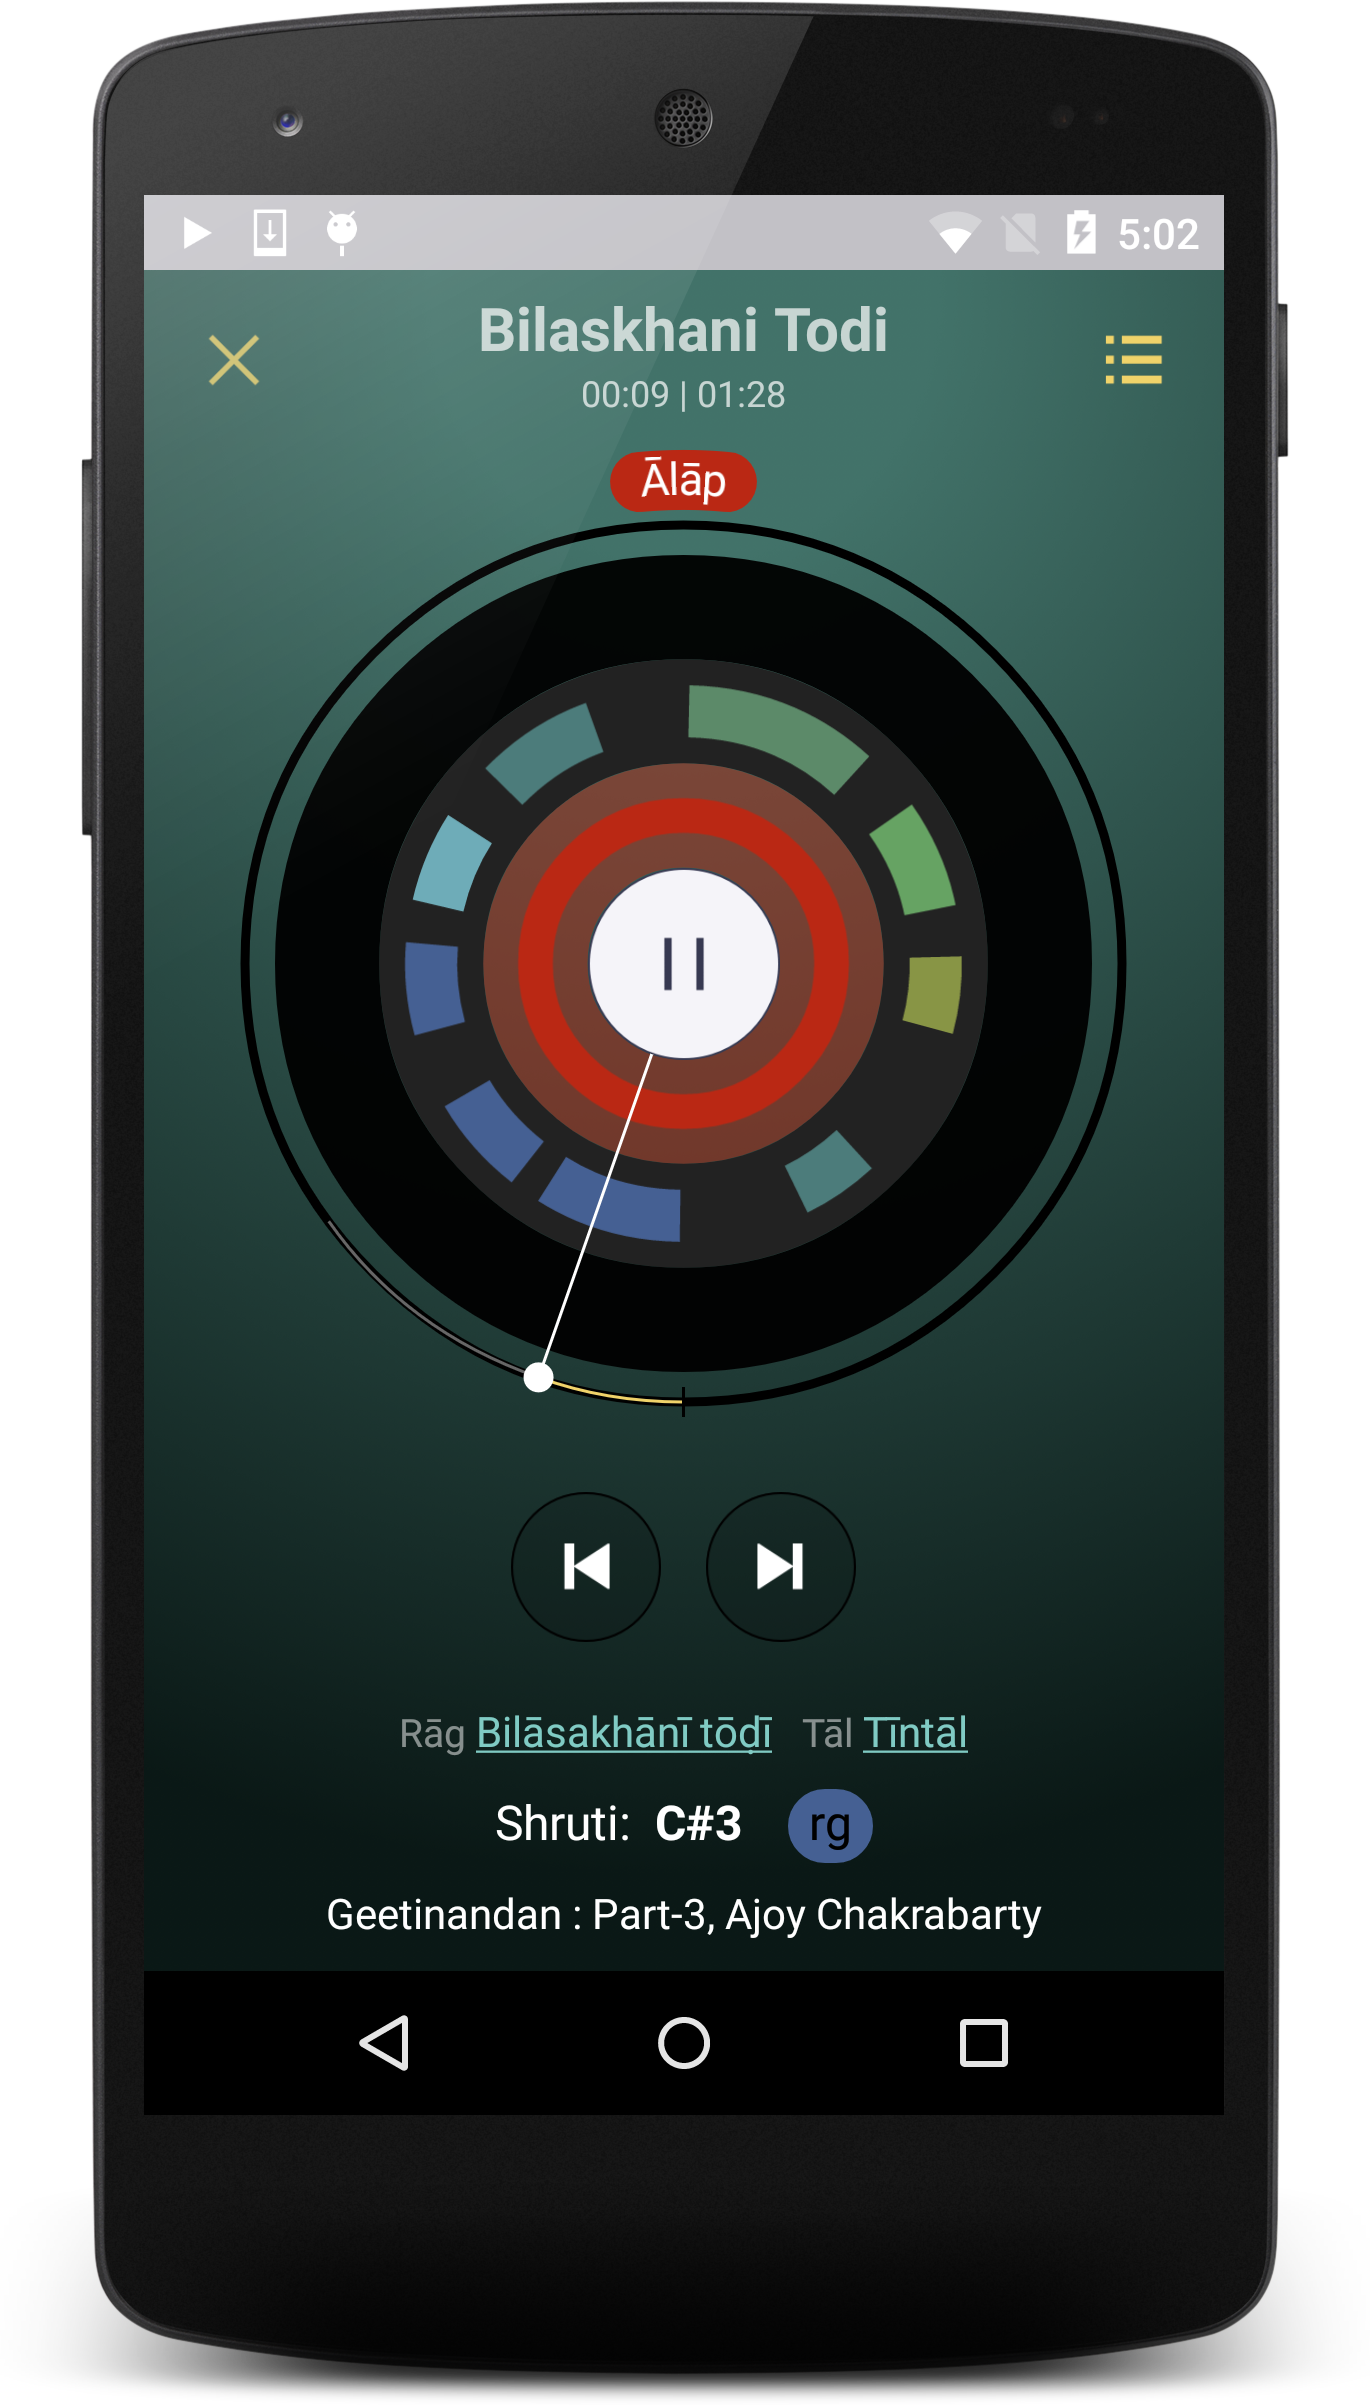
\includegraphics[width=\figSizeNinety]{ch08_applications/figures/saraga2.png}
		\caption{\Gls{alap} section (zoomed in)}
		\label{fig:saraga_alap_section}
	\end{subfigure}
	\caption[Screenshots of the mobile application, \gls{saraga}]{Screenshots of the mobile application, \gls{saraga}, showing a music piece of Hindustani music. (a) shows the entire music piece, (b) shows the \gls{alap} section in the piece. Melodic phrases are marked by the colored arches. Tonic (\gls{shruti}) of the recording is shown at the bottom along with the current playing melodic phrase.}
	\label{fig:saraga_screens}
\end{figure}

In~\figref{fig:saraga_screens}, we show a screenshot of the recording screen in \gls{saraga} playing a music piece\footnote{\url{https://musicbrainz.org/recording/3124479b-5118-4cf3-823f-8fefad45e586}} in Hindustani music. In~\figref{fig:saraga_screens}\,(a), the entire music piece is visualized. Information regarding the sections, melodic patterns, and the \gls{sama} locations is displayed through the concentric circles as indicated in the screenshot. As the playback advances in time along the circle, these descriptors are highlighted based on the current time. For example, in~\figref{fig:saraga_screens}\,(a), the melodic phrase ``rg'' is being sung in the piece, which is highlighted at the bottom of the screen. Since music performances in \gls{iam} can last long (sometimes up to an hour), \gls{saraga} interface allows to tap and zoom into a particular section. An example of this is shown in~\figref{fig:saraga_screens}\,(b), wherein the \gls{alap} section is selected. Furthermore, a user can also tap on a particular melodic pattern to go to a screen, where all the occurrences of that pattern in the recording are shown together. These functionalities facilitate a user to better understand the structures of different musical facets in a piece of \gls{iam}. In addition to these descriptors, there is accompanying data shown at the top and the bottom of the screen, which includes editorial metadata and \gls{shruti} (tonic) information. The text strings corresponding to the musical concepts (\gls{raga} and \gls{tala}) are hyper-linked to their respective pages, where that music concept is described using a set of representative audio examples. 



\subsubsection{\glsentrytext{riyaz}}
\label{sec:riyaz}

\begin{figure}
	\begin{subfigure}{\textwidth}
			\centering
		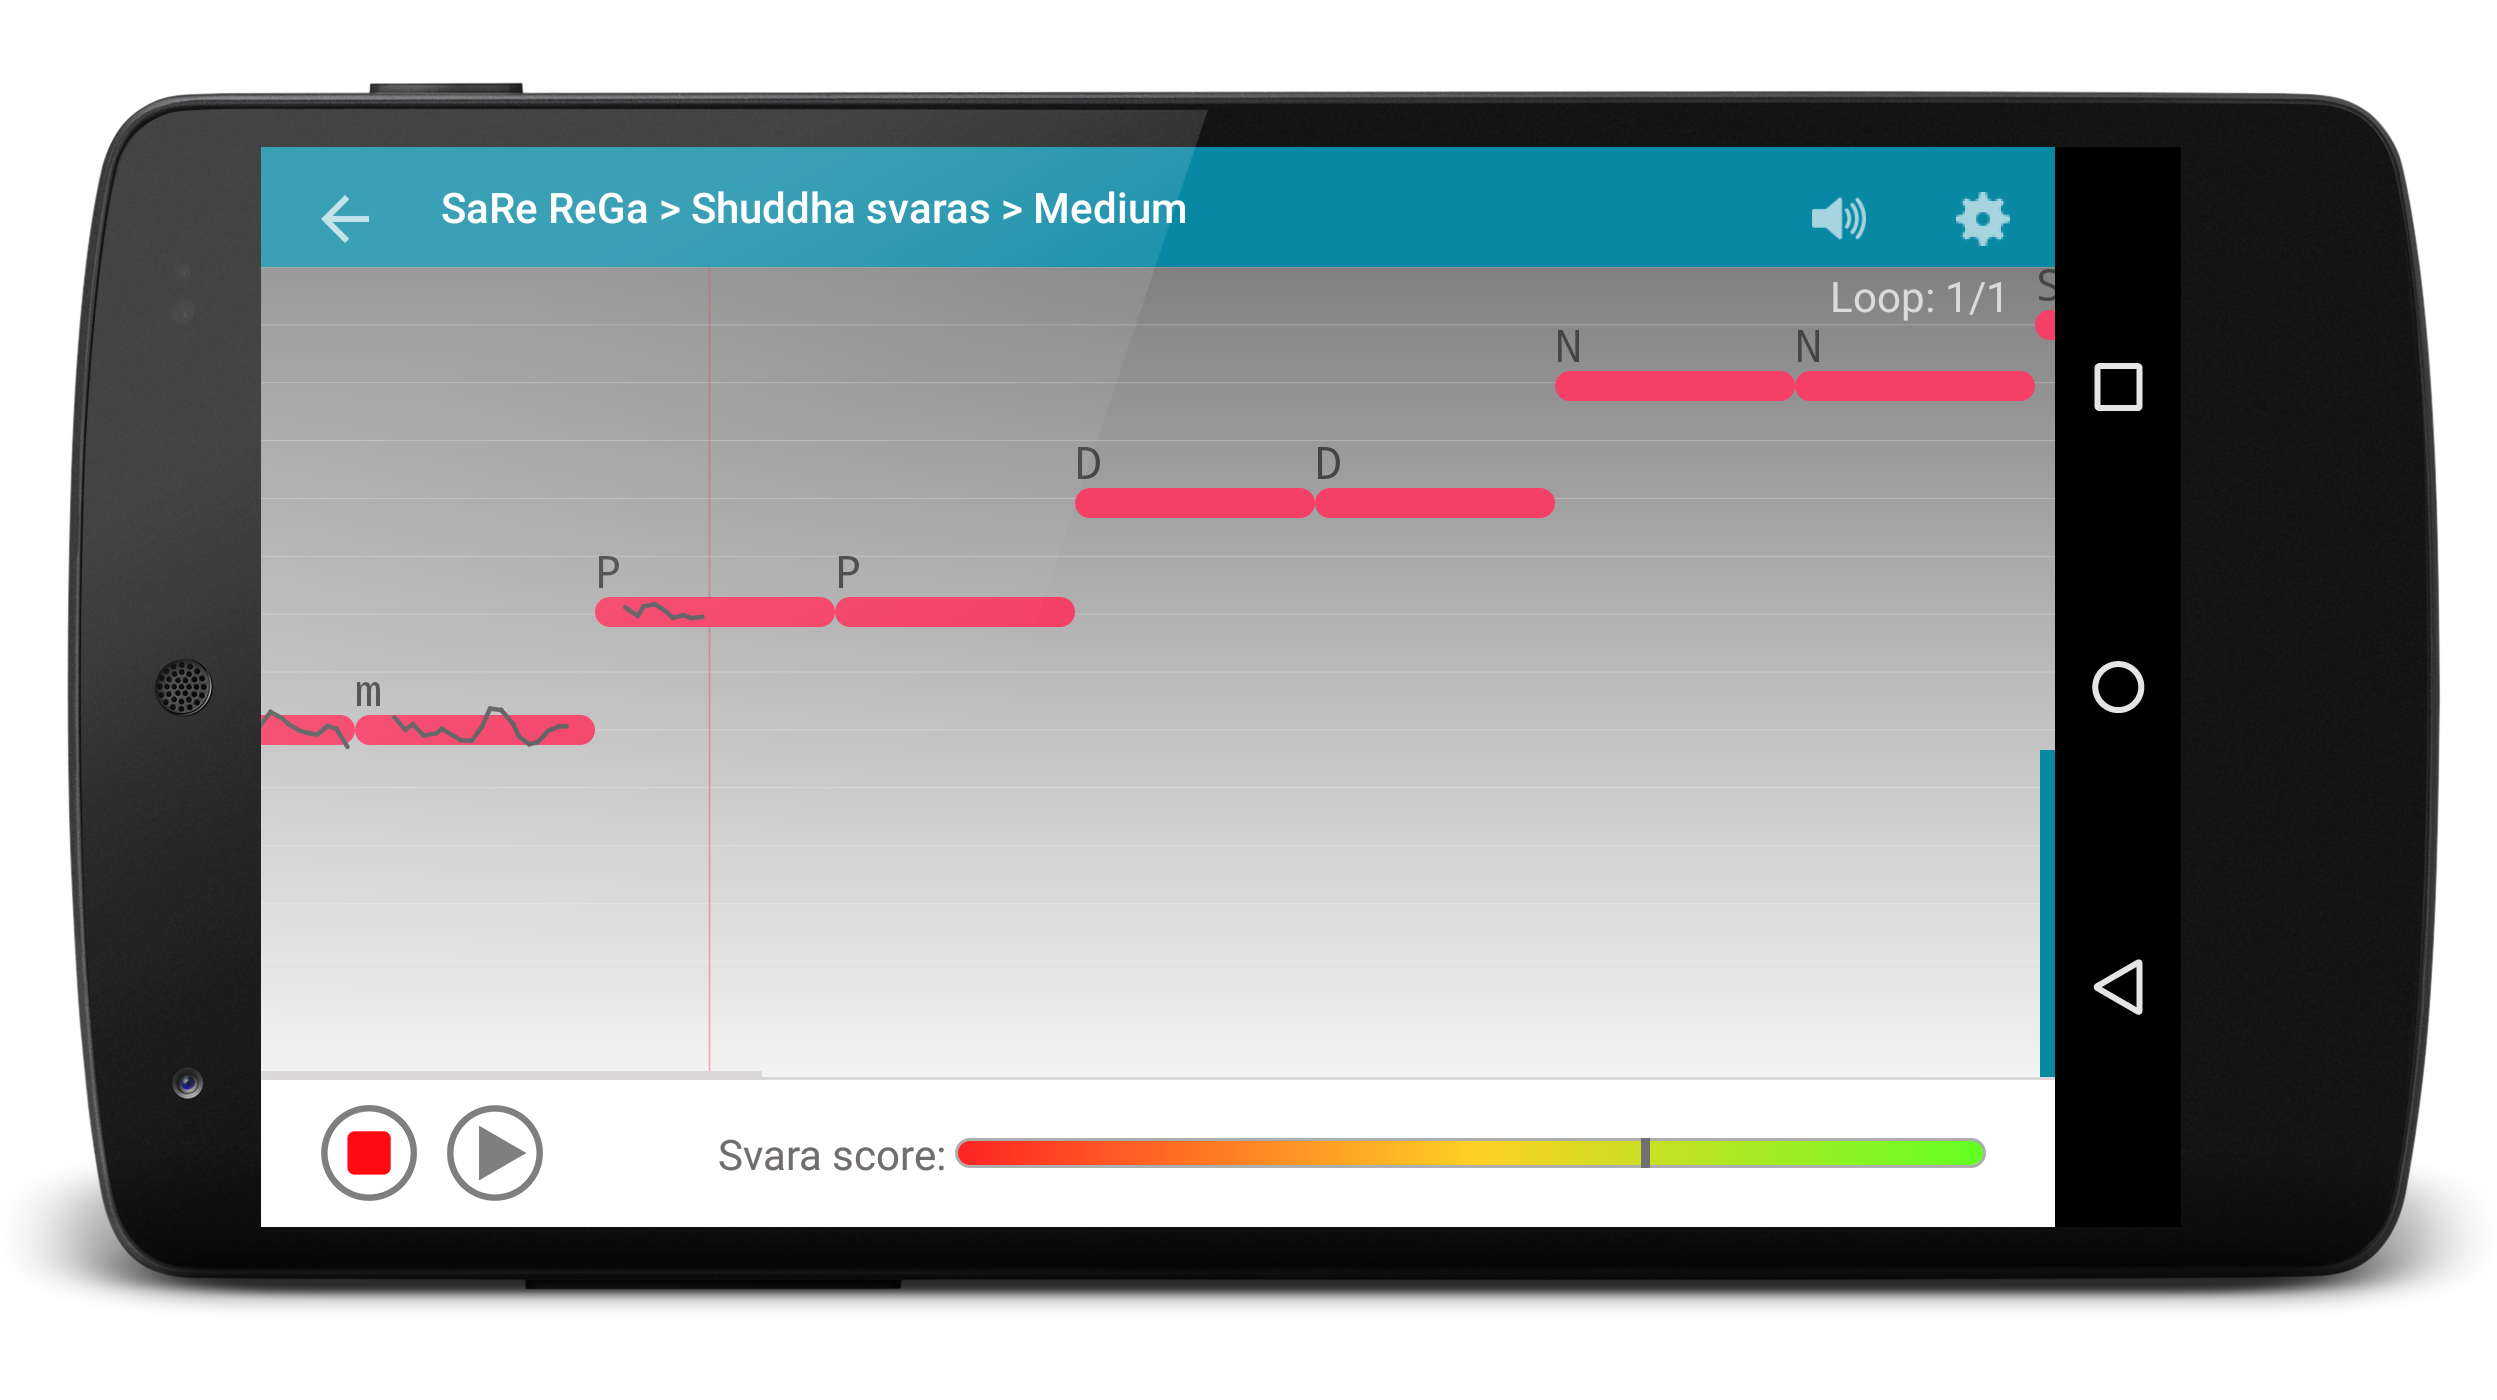
\includegraphics[width=\figSizeSeventy]{ch08_applications/figures/riyaz1.png}
		\caption{Evaluation screen}
		\label{fig:riyaz_evaluation_screen}
	\end{subfigure}
	\begin{subfigure}{\textwidth}
			\centering
		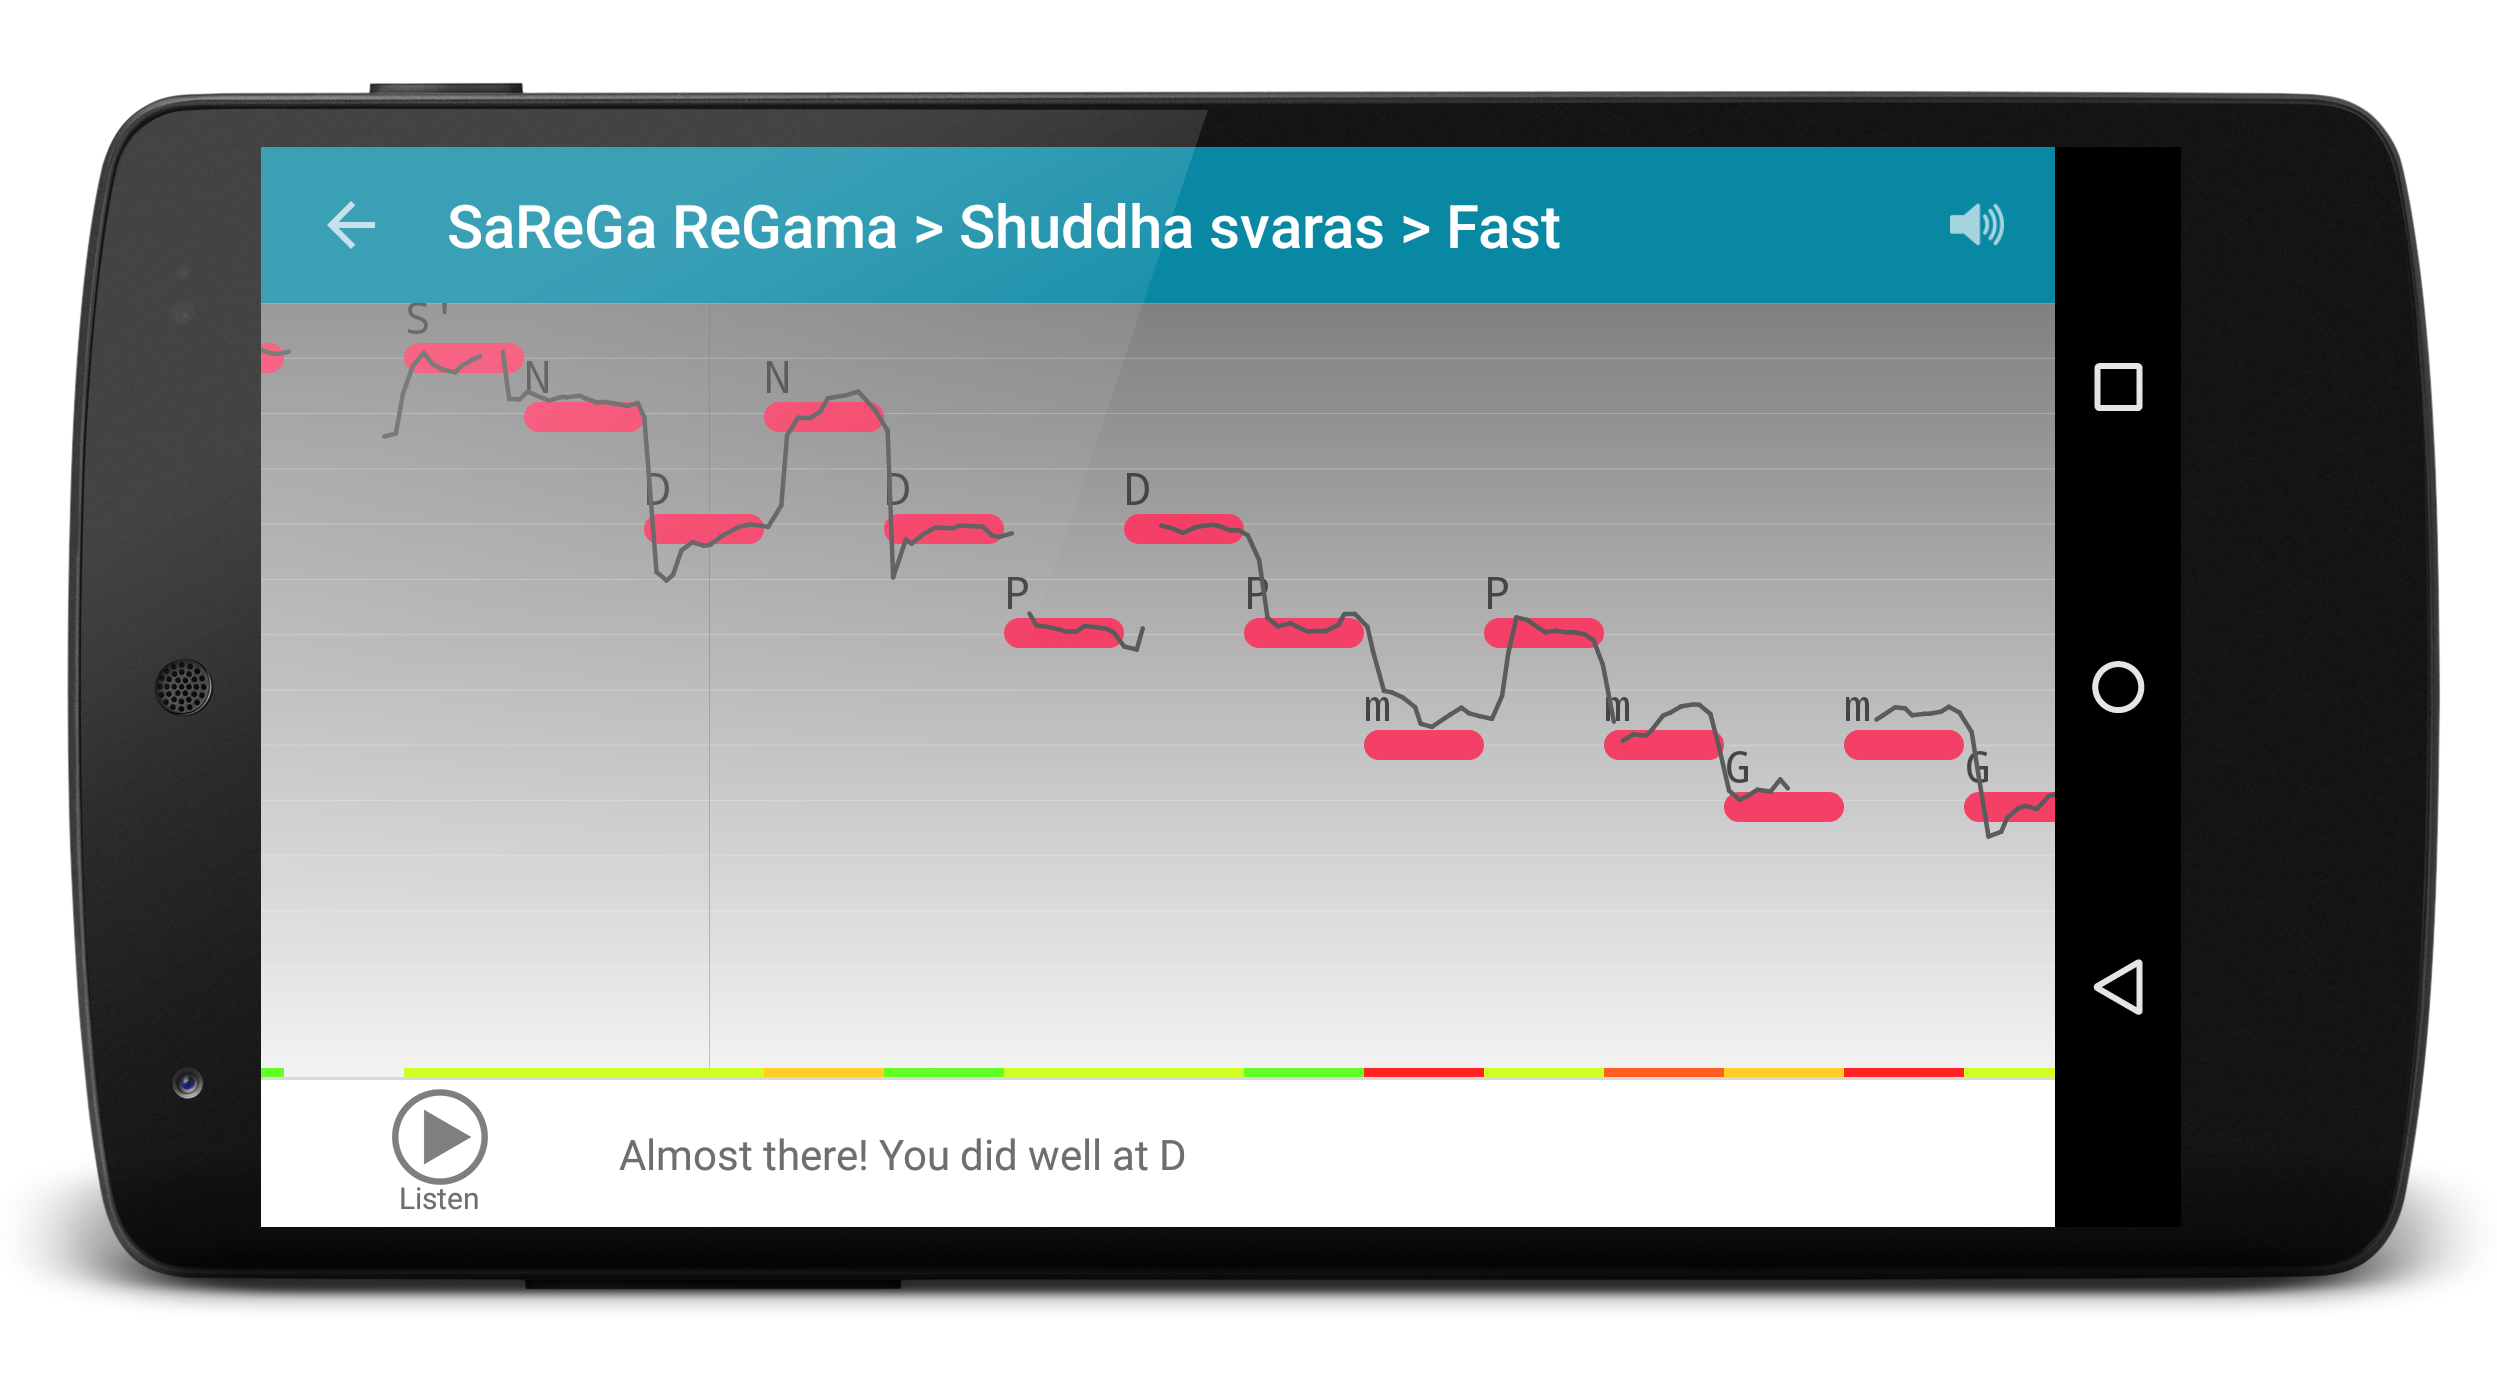
\includegraphics[width=\figSizeSeventy]{ch08_applications/figures/riyaz2.png}
		\caption{Feedback screen}
		\label{fig:riyaz_feedback_screen}
	\end{subfigure}
	\caption{Screenshots of the mobile application, \gls{riyaz}.}
	\label{fig:riyaz_screens}
\end{figure}

\gls{riyaz} is a mobile application that aims to facilitate music learning for students of \gls{iam} by making their practice sessions more efficient. This is achieved by simulating a student-teacher interaction in which learning happens through imitating the musical exercises build by processional musicians. The application performs singing assessment and provides a detailed feedback, wherein it highlights the mistakes and gives suggestions to improve. In~\figref{fig:riyaz_screens}\,(a), we show the main evaluation screen of \gls{riyaz}, where a user can visualize, in real-time, the pitch track and the computed \gls{svara} score. After a practice session, a detailed feedback is provided as shown in~\figref{fig:riyaz_screens}\,(b). Note that, \gls{riyaz} is a work in progress with a prototype version already available at the time of writing this thesis. Currently there are 1500+ users with 20,000+ user sessions. 


\section{Demos}
\label{sec:demos}

We now proceed to present two elementary web-based applications that demonstrate the outcome of our pattern discovery approach. In addition, we also present \gls{ragawise}, a prototype web application for real-time \gls{raga} recognition. 

\subsection*{Demo1: Melodic Patten Discovery}

One of the motivations behind performing pattern discovery is to explore novel relationships in the data and extract new knowledge. However, it is a challenging task to evaluate these aspects in a quantitative evaluation setup, wherein available ground-truth (typically comprising annotations from an expert) is used as a basis to measure the quality of the output. It becomes even more challenging when these unsupervised analyses are performed on large datasets, such as in our case, in which obtaining the ground-truth becomes practically unfeasible. In the study presented in~\secref{sec:patterns_melodic_pattern_discovery}, we performed melodic pattern discover in audio collections of Carnatic music comprising nearly 365\,hours of music. Though we performed a quantitative evaluation using a randomly sampled subset of the output, the evaluation numbers do not convey much in terms of the musical novelty of the patterns. 

In order to facilitate informal evaluations, take feedback from musicians, identify novel outcomes, and eventually, to improve the quality of the output of our pattern discovery methods we built two web-based applications that expose the discovered melodic patterns. 

\begin{figure}
	\begin{center}
		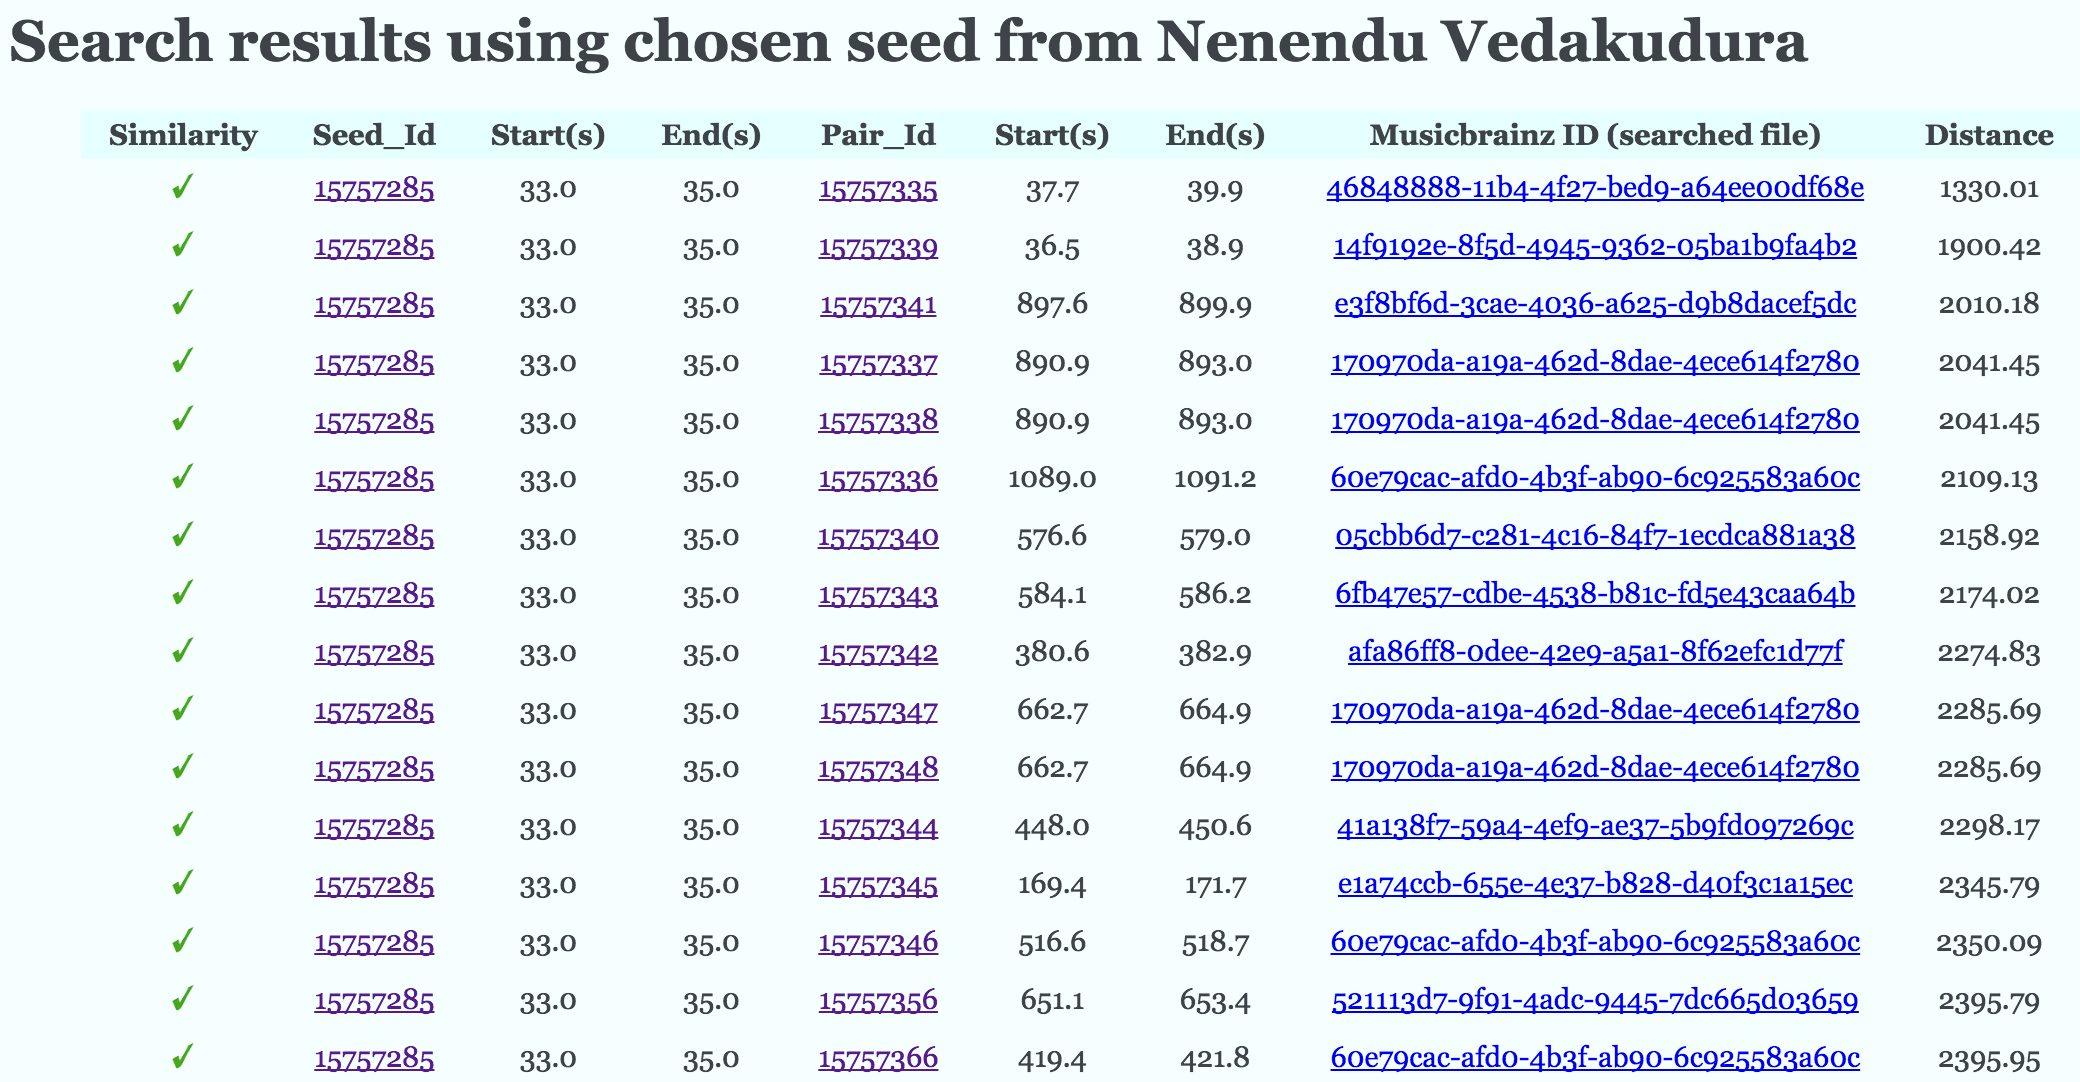
\includegraphics[width=\figSizeHundred]{ch08_applications/figures/patternBrowsing1.png}
	\end{center}
	\caption[A web demo for navigating through the discovered melodic patterns]{Screenshot of a web demo for navigating through the discovered melodic patterns organized by artists, releases and recordings.}
	\label{fig:browser_patterns}
\end{figure}

Our first demo enables a user to browse through all the melodic patterns discovered in the study reported in~\secref{sec:patterns_melodic_pattern_discovery}. Since determining a meaningful similarity threshold is in itself a challenging task, we selected a fixed number of closest pattern matches in the output. To recall, 25~closest seed pattern pairs were selected within a recording, and for each seed pattern its 200~closest neighboring patterns were selected across the entire music collection (\secref{sec:patterns_discovery_method}). This resulted in around 15~million patterns for our audio collection that comprises 1764~recordings. This demo allows us to navigate through all the recordings in the collection, fetch all the seed patterns for a recording, and for each seed pattern, fetch their closest patterns from the entire music collection. In~\figref{fig:browser_patterns}, we show a screenshot of a page where a list of closest melodic patterns for a seed pattern is displayed. All the listed melodic patterns can be played and listened to. From the column that specifies the \glspl{mbid} of the recordings of the retrieved patterns, we readily notice that these patterns are from different recordings (\figref{fig:browser_patterns}). These recordings are from different artists with different tonic pitches, and even across vocal and instrumental music. With such an interface it becomes easy to assess the quality of the discovered melodic patterns and to identify musically novel patterns. 

\begin{figure}
	\begin{center}
		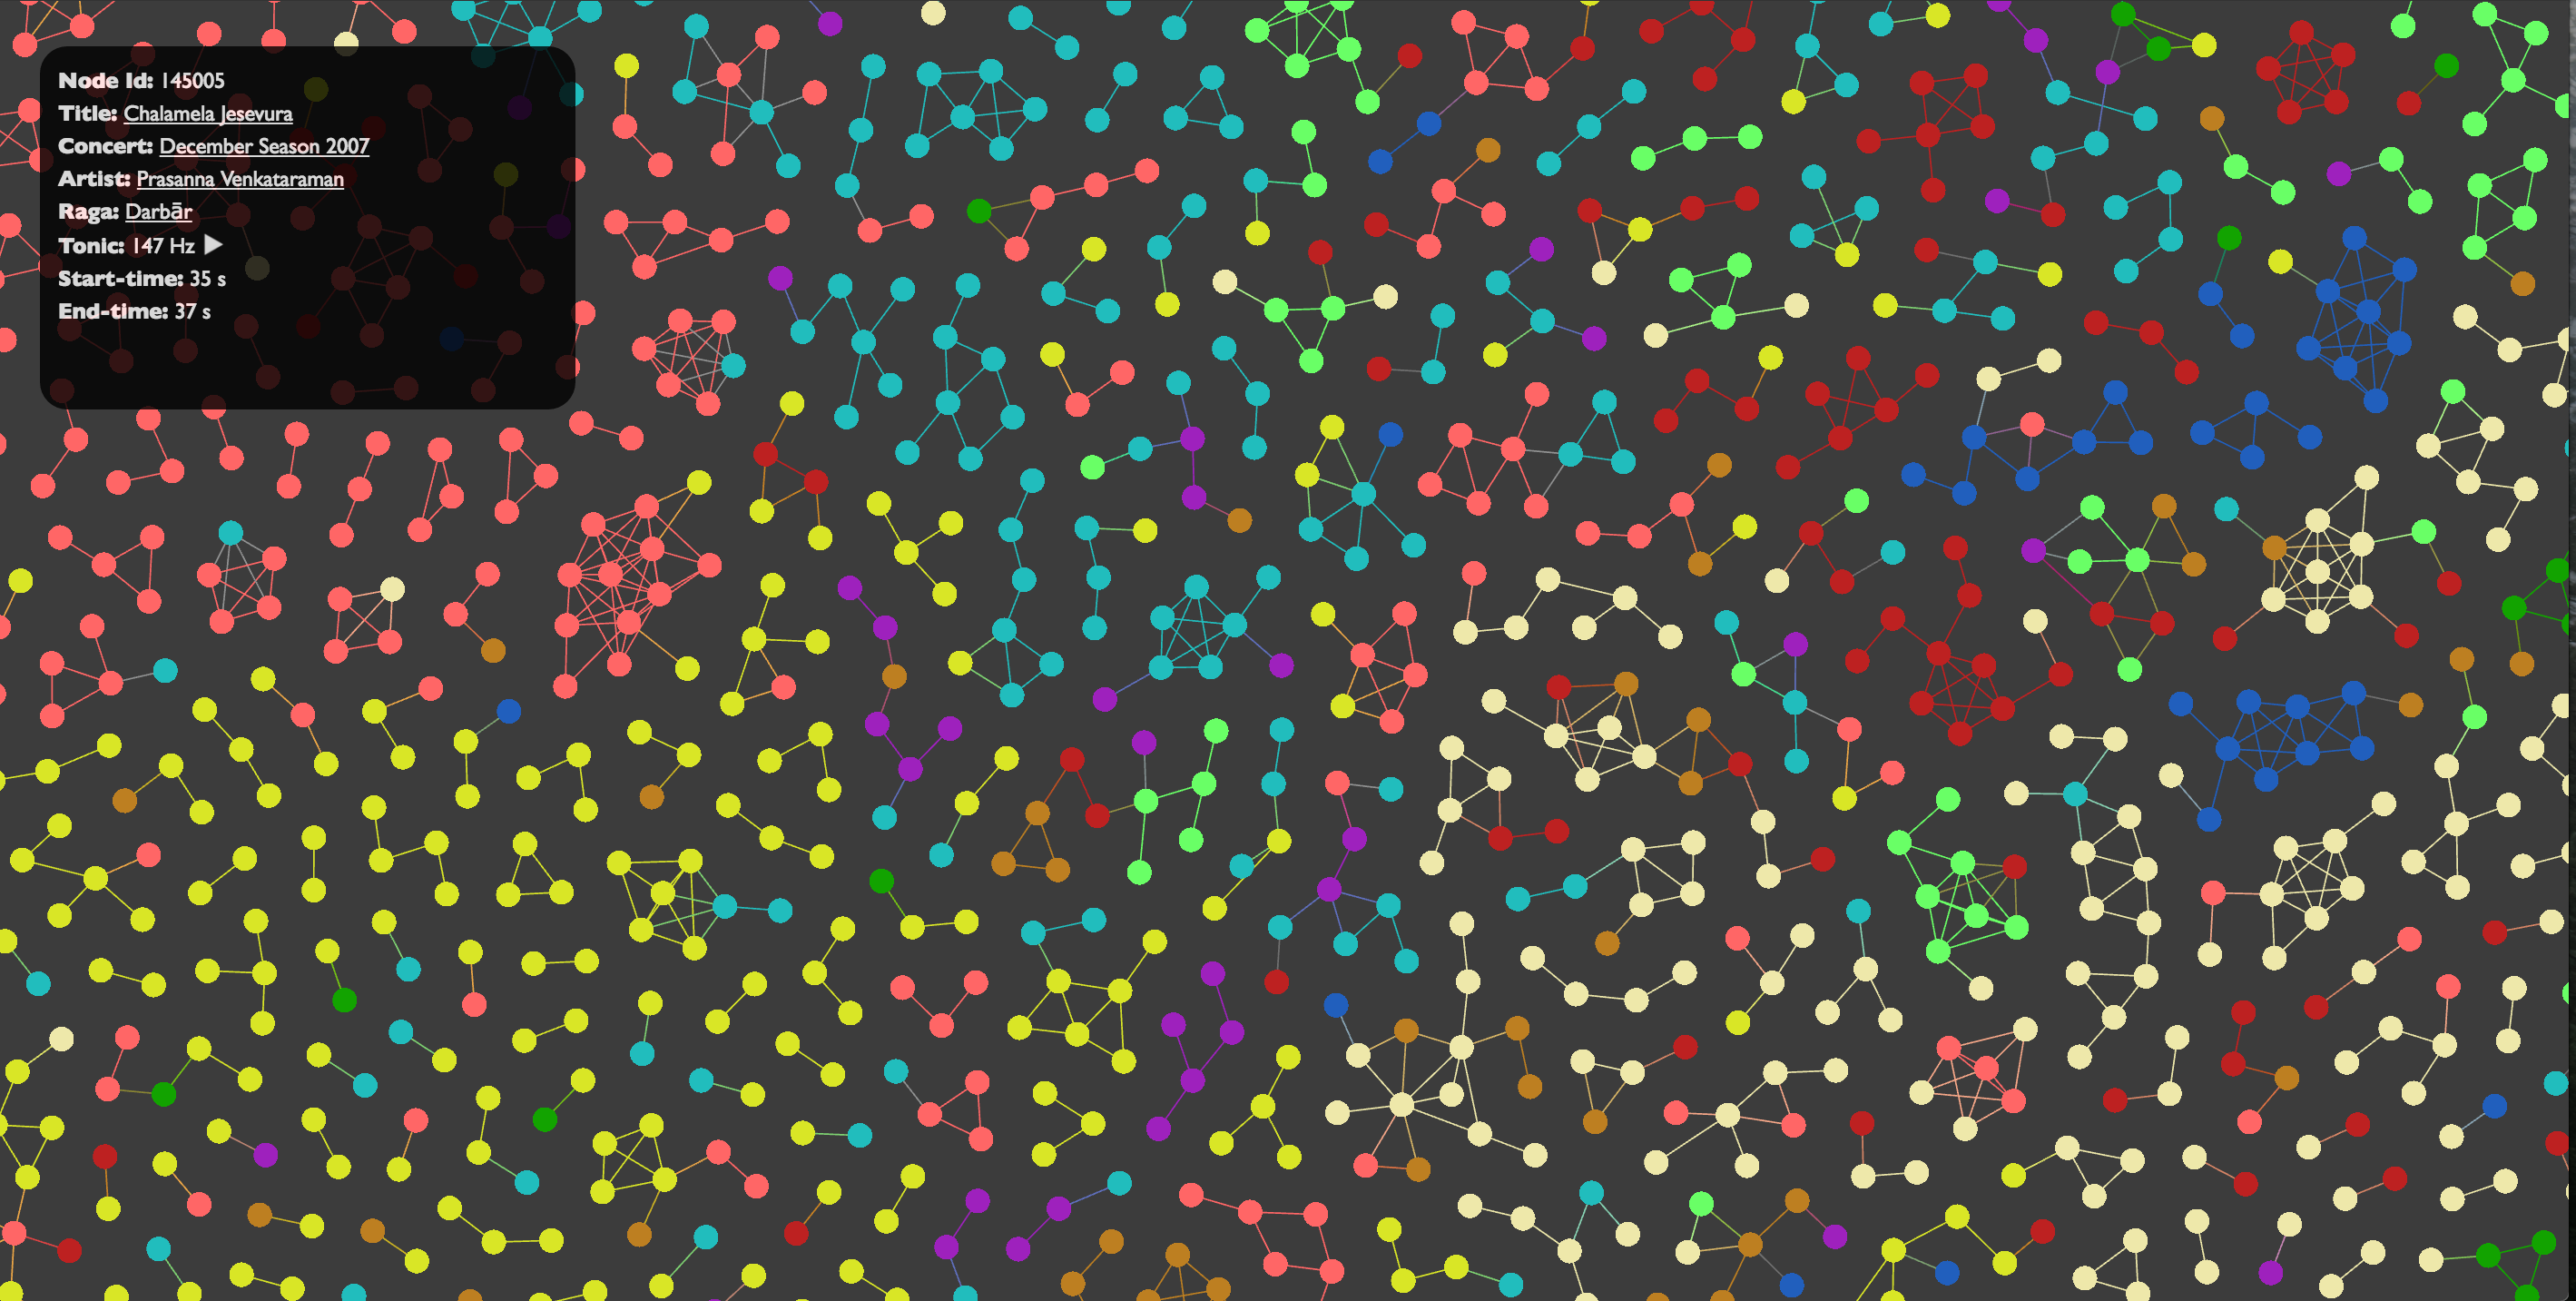
\includegraphics[width=\figSizeHundred]{ch08_applications/figures/patternNetwork1.png}
	\end{center}
	\caption[A web demo of a network of the discovered melodic patterns]{Screenshot of a web demo of the network of the discovered melodic patterns. Colors indicate different \glspl{raga}.}
	\label{fig:network_patterns}
\end{figure}

The demo described above presents the melodic patterns by structuring them in a hierarchical manner (according to the editorial metadata of the collection), which is useful to look for patterns in a particular music piece or by a particular artist. An alternate way to present these patterns and their relationships is through a network visualization. Such a visualization makes it easier to identify interesting and novel relationships between different music pieces, artists, and \glspl{raga}. In~\figref{fig:network_patterns}, we show a screenshot of our second demo that presents a network visualization of the discovered melodic patterns. These melodic patterns are the ones obtained in the study described in~\secref{sec:patterns_characterization_of_melodic_patterns}. Note that, in this study we employed a network analysis to also determine a melodic similarity threshold, as a result of which we only retain the musically meaningful connections between the melodic patterns. The nodes of the network are the melodic patterns and the edges represent a binary melodic similarity between the nodes. In addition, for each node we also provide the accompanying information of the audio recording from which it is extracted (\figref{fig:network_patterns}, top-left corner). Furthermore, we also provide an option to play a tone that corresponds to the tonic of the recording. This helps to establish the tonal context of the melodic pattern. Both the web demos described above provide useful insights in to the outcome of our pattern discovery approach. They are made available online (\appref{app:resources}). 


\subsection*{\glsentrytext{ragawise}: Real-time Raga Recognition}
\label{sec:ragawise}

In~\chapref{chap:raga_recognition}, we described our computational approaches for \gls{raga} recognition. Our objective was to develop novel methods to obtain a \gls{raga} label for a recorded music performance. As mentioned earlier, there are several applications of these methods such as automatic \gls{raga} annotation of large audio archives, \gls{raga}-based music retrieval, establishing meaningful similarity measures across recordings and music pedagogy. In this section we present a prototype web application, \gls{ragawise}, which demonstrates the usability of such systems in the context of music pedagogy. 

\gls{ragawise} is a real-time \gls{raga} recognition prototype system~\citep{ragawise}. It uses \gls{pcp}, pitch transitions and melodic patterns to recognize \gls{raga} from an incoming audio stream. For each \gls{raga} it stores a dictionary of the \glspl{svara}, \gls{svara} transitions, and typical melodic patterns. It processes the input vocals in real-time to estimate pitch, and subsequently performs melody transcription. The likelihood of each \gls{raga} is updated in real-time based on the identified of \gls{raga} elements in the melody. In order to highlight the melodic events that are characteristic of a \gls{raga}, a dynamic visualization of the evolution of the likelihood of all the \glspl{raga} is performed. We present a screenshot of \gls{ragawise} in~\figref{fig:ragawise}, where different panels are marked by blue arrows. In the top panel (arrow~1) we display the transcribed melody symbols (\glspl{svara} in this case) using the pitch track obtained in real-time (arrow~2). We continuously process the transcribed melody to detect the presence of different melodic elements, and once detected, we highlight the associated \glspl{raga} (arrow~3,4,5). We also compute a cumulative salience score of each \gls{raga} based on the frequency of the detected melodic elements (arrow~6).

Note that, building \gls{ragawise} was a team effort done as a part of the hackday, HAMR, in ISMIR-2015. It is done in collaboration with Kaustuv Kanti Ganguli, Swapnil Gupta and Ajay Srinivasamurthy. 

\begin{sidewaysfigure}
	\begin{center}
		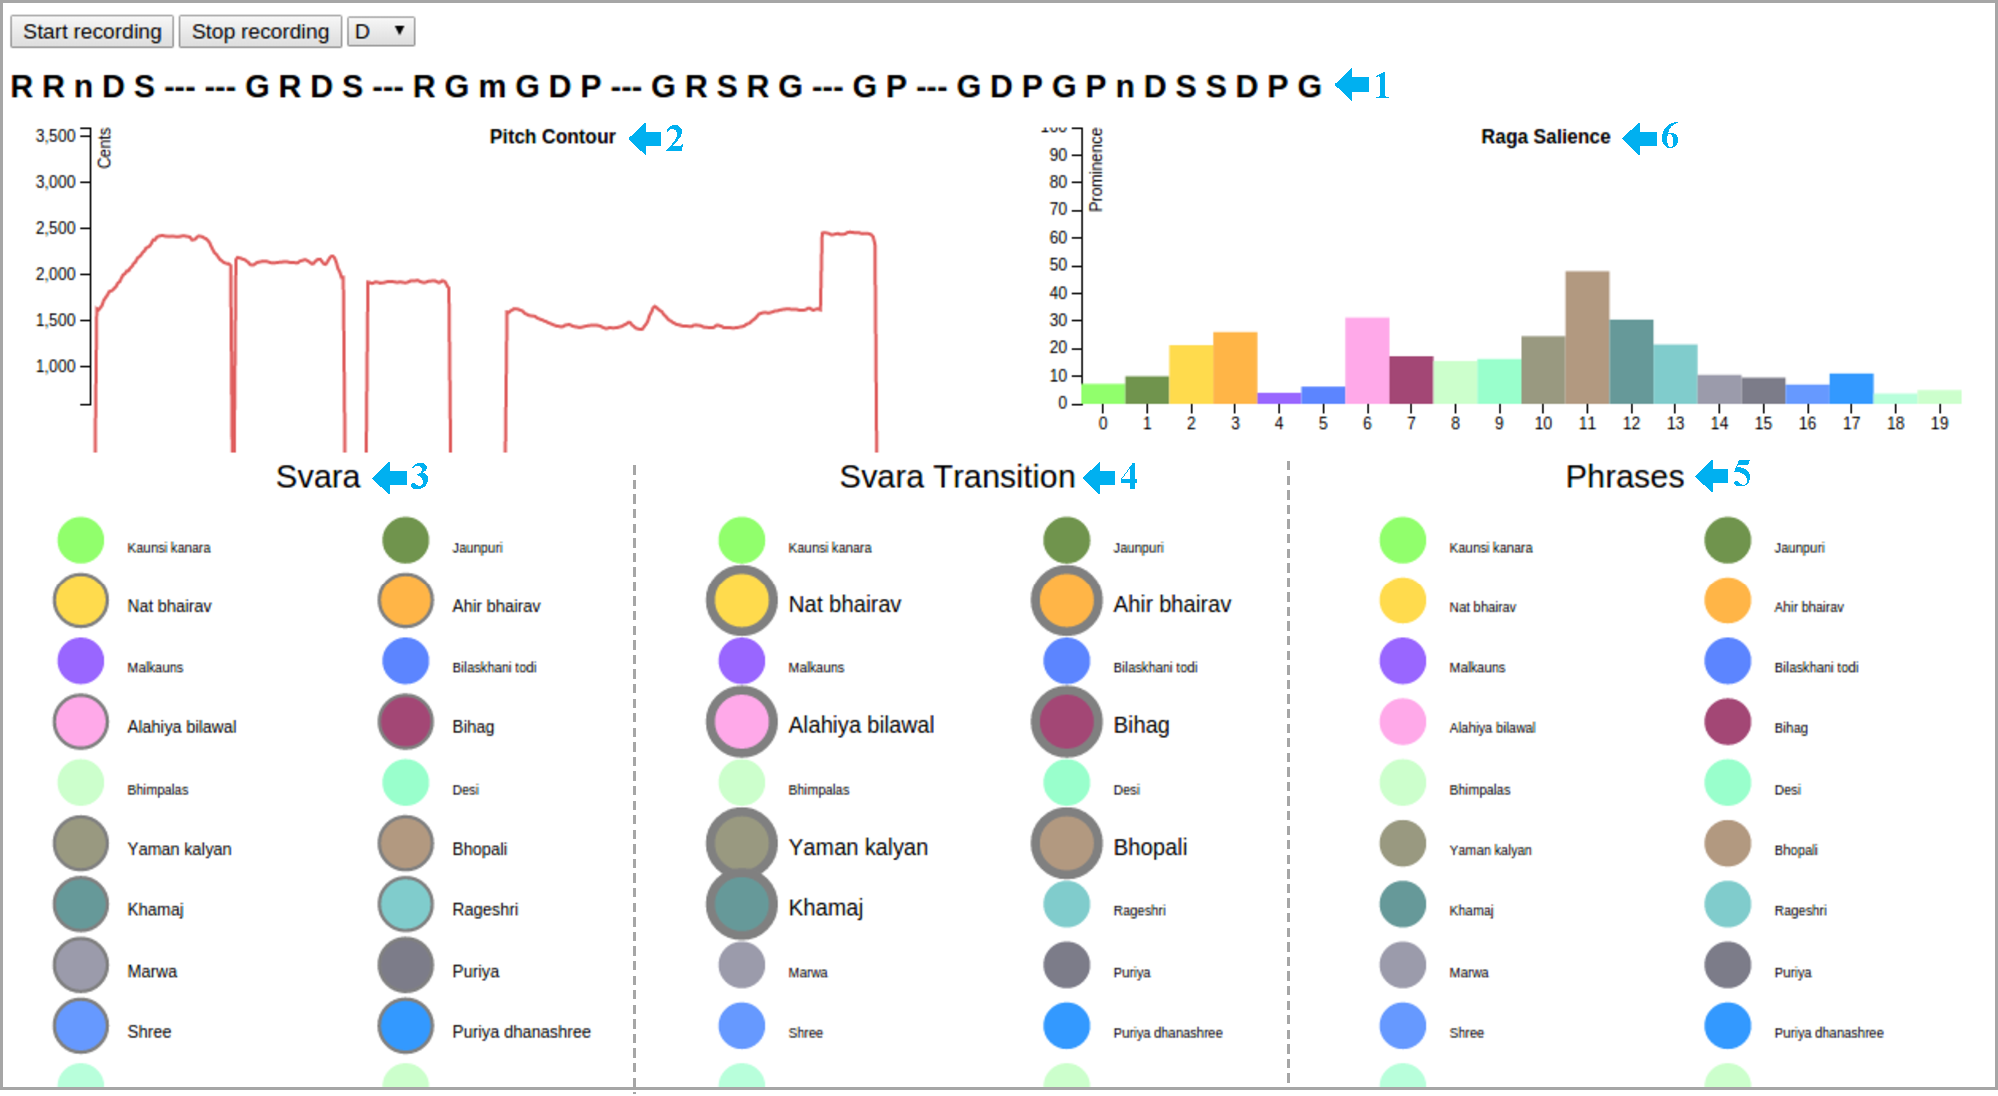
\includegraphics[width=\figSizeHundred]{ch08_applications/figures/ragawise.pdf}
	\end{center}
	\caption[Screenshot of \gls{ragawise}]{Screenshot of \gls{ragawise}, which illustrates real-time pitch tracking, melody transcription and \gls{raga} salience evolution. Bottom panel shows a list of \glspl{raga} for each melodic element (\gls{svara}, \gls{svara} transition and melodic patterns). \Glspl{raga} for which a particular melodic element is detected in the audio stream are highlighted.}
	\label{fig:ragawise}
\end{sidewaysfigure}


\section{Computational Musicology}

The research work presented in this thesis paves the way for a number of studies in the context of computational musicology in \gls{iam}, which can be performed at a large scale using corpora of recorded performances. We provide here an example of our preliminary work in this direction. 

As mentioned, \gls{iam} is primarily an improvisatory music tradition, wherein compositions merely serve as the skeleton of a performance. However, at the same time, melodies are constructed in adherence with the \gls{raga} grammar, and therefore, they are bound by certain rules (or conventions). This fine distinction between what is `fixed' and what remains `free' is not clearly defined and is implicitly acquired by music students through years of musical training. With this as our motivation, in~\cite{kaustuv_ismir_2016}, we propose methods to discover melodic structures in recorded performances of \gls{iam}. In this study, we utilized several outcomes of the methods described in this thesis such as melody representations, tonic normalization and \gls{nyas} segmentation. We studied five different aspects related with the temporal evolution of melody in a music piece: the overall coarse evolution of melody in time, the transition characteristics of consecutive \gls{nyas} \glspl{svara}, the relationship between the functional roles of the \glspl{svara} and their duration in melody, the duration and position of \glspl{svara} in melody, and the presence of the possible pulsation in \gls{alap} melodies. 

\begin{figure}
	\begin{center}
		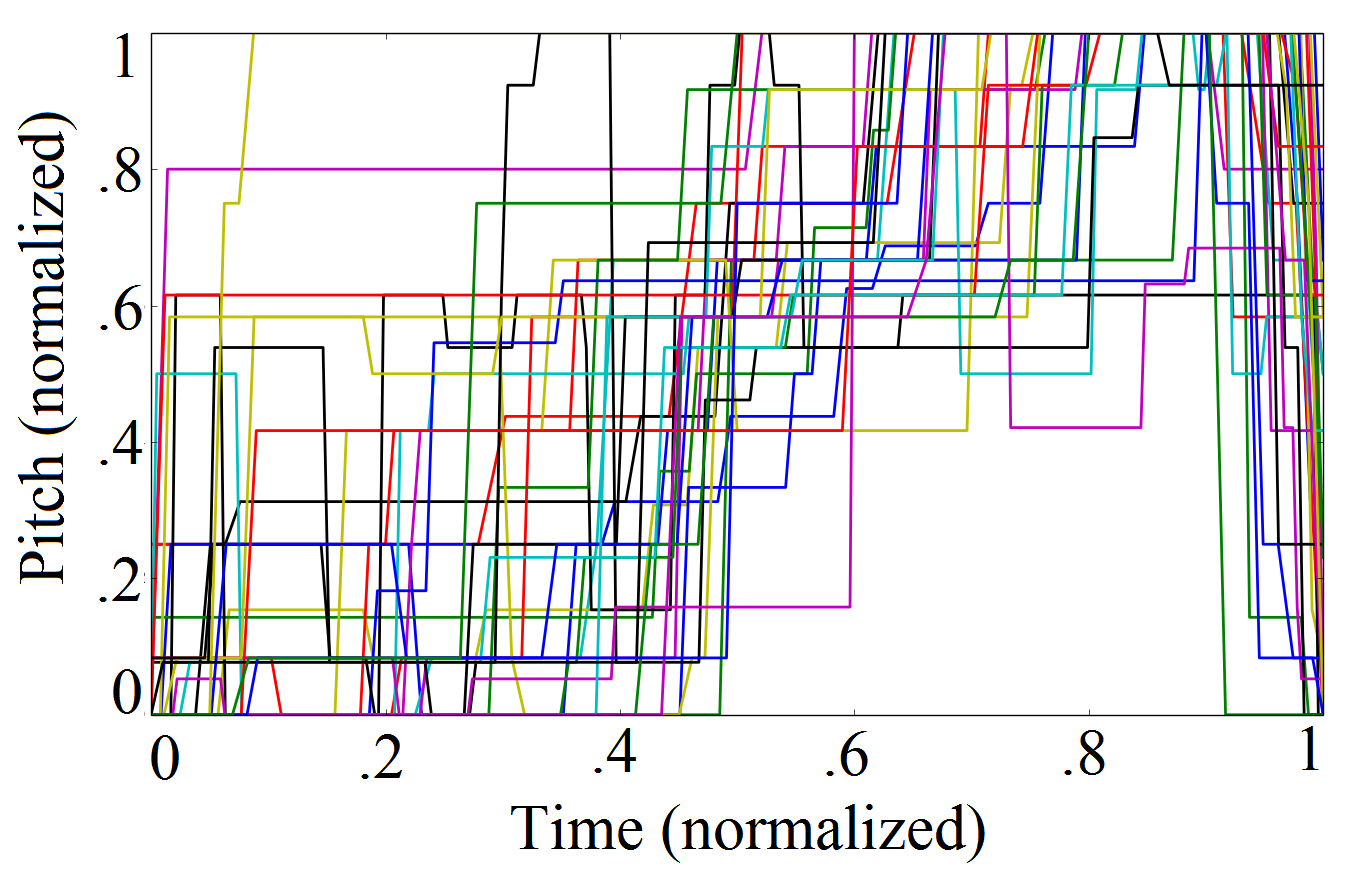
\includegraphics[width=\figSizeSeventy]{ch08_applications/figures/Fig-5.png}
	\end{center}
	\caption{Temporal evolution of long-term averaged melody contours for 37 performances. The length of the performances are normalized.}
	\label{fig:temporal_evolution}
\end{figure}

One of the interesting results from this study is related to the overall evolution of melody in a music piece. We found that, irrespective of the functional roles of the \glspl{svara}, they are explored in melodies in a linear manner by an artist, starting from the lowest frequency \gls{svara} going all the way to the highest. Interestingly, this trend appears to be largely independent of the duration of the performance. In~\figref{fig:temporal_evolution}, we illustrate this pattern by showing the trajectories of the highest salience bin in a long-time averaged pitch histogram computed across breath-phrases\footnote{Segment of the melody between two breath pauses (>300\,ms) by a singer}. 

\begin{figure}
	\begin{center}
		\ifdefined\PRINTVER
			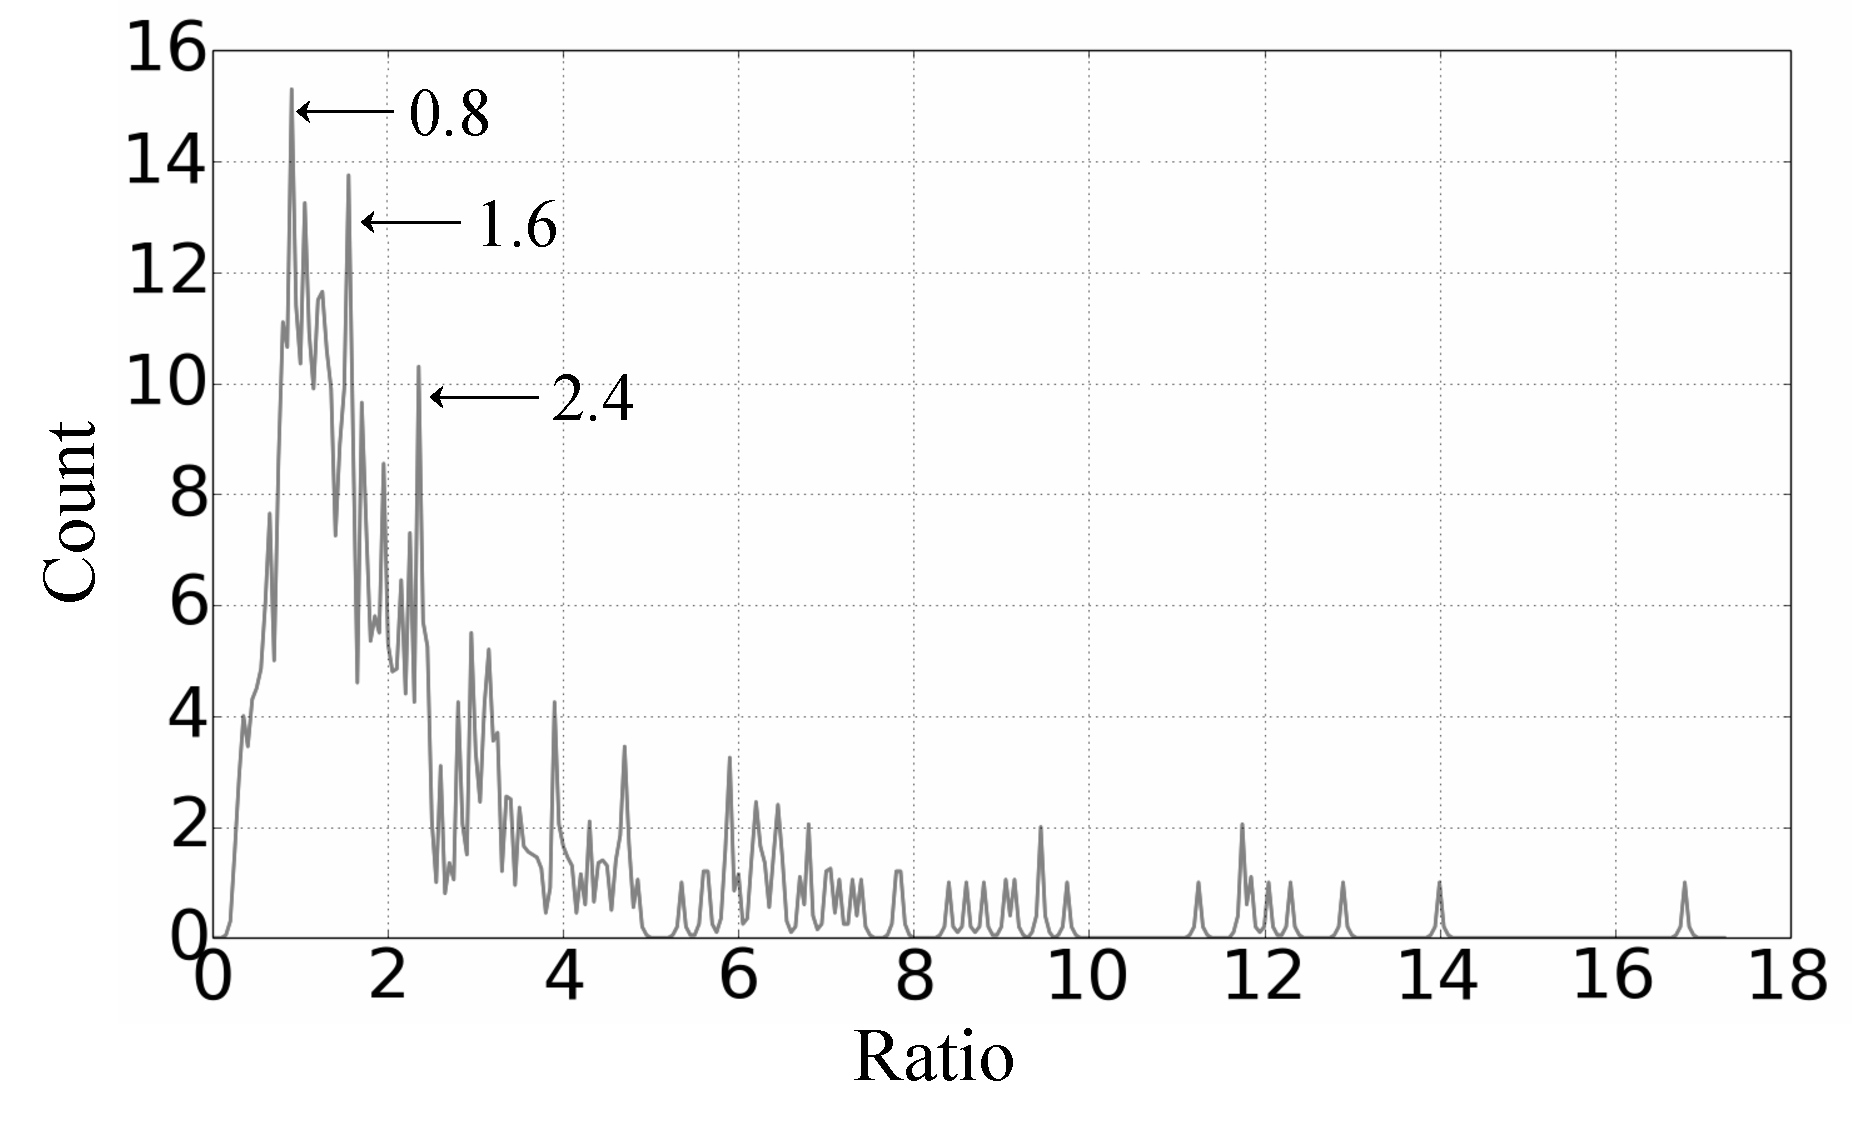
\includegraphics[width=\figSizeSeventy]{ch08_applications/figures/Fig-8_BW.pdf}
		\else
			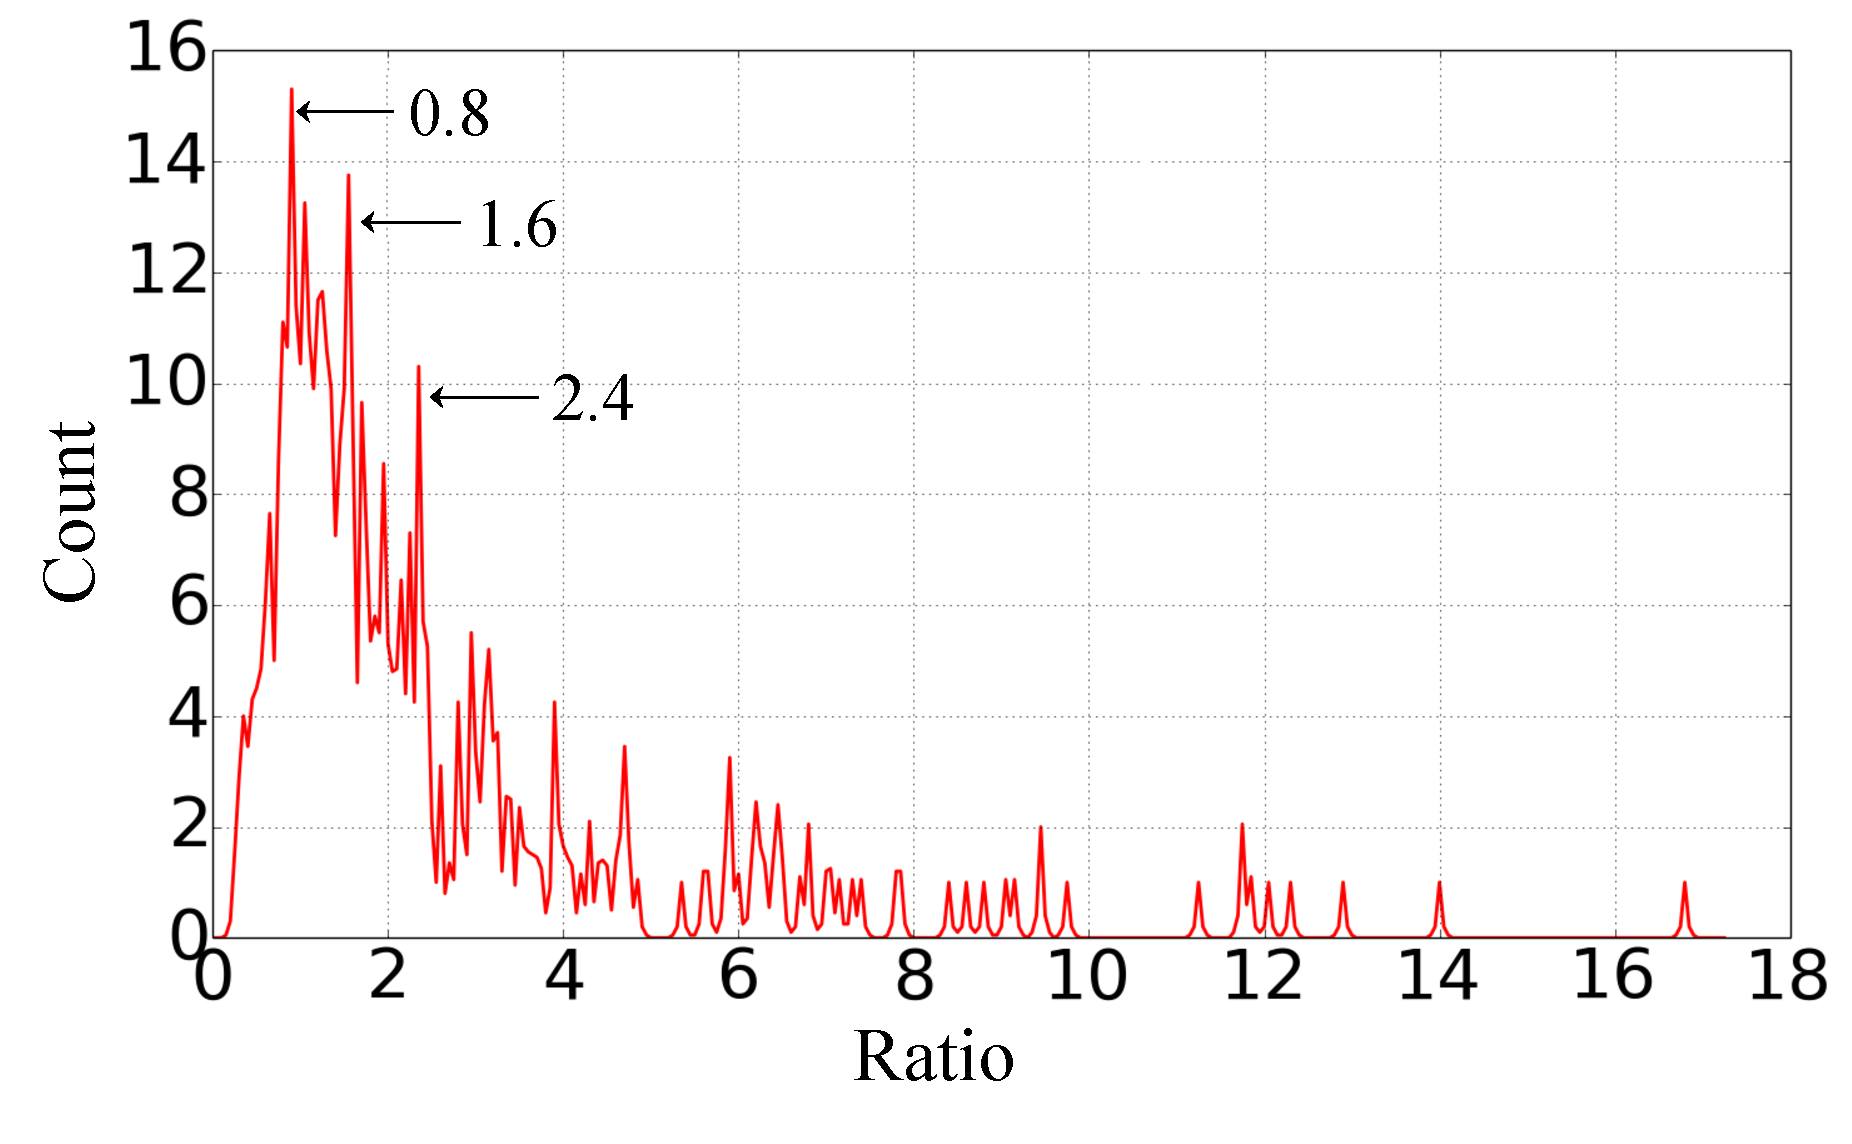
\includegraphics[width=\figSizeSeventy]{ch08_applications/figures/Fig-8.pdf}
		\fi
	\end{center}
	\caption{Histogram of the ratio of the inter-onset-intervals of salient \glspl{svara} across breath-phrases.}
	\label{fig:pulsation_example}
\end{figure}

Another interesting result is that although the \gls{alap} section is unmetered, a histogram of the ratio of the inter-onset-intervals between the salient \glspl{svara} across breath-phrases shows strong pulsation (\figref{fig:pulsation_example}). This corroborates with the existing musicological discussion that there is indeed a pulsation in \gls{alap} melodies. For a detailed description of the methodology used in the analysis and comprehensive results of the study, we refer to~\cite{kaustuv_ismir_2016}.

\section{Summary}
\label{sec:applications_summary}

In this section, we presented some concrete examples of different applications of our work in several contexts such as computational musicology, enhance music listening applications, and pedagogical tools for \gls{iam}. We presented Dunya, a research tool that comprise all the data and software tools developed in the CompMusic project. We briefly described two different ways to access the research corpora compiled in the project. Using this tool and the compiled corpora, a number of datasets can be created to study different aspects of \gls{iam}. Subsequently, we presented web-based demos that enable a user to browse and listen to the melodic patterns discovered by our approach through an intuitive user interface. Listening to and analyzing the relationships between these melodic patterns provide useful insights, which can be looped back to further improve our system. We also presented a web prototype of \gls{ragawise} that demonstrates the utility of an automatic raga-recognition system a real-time setup, which can further be exploited to develop tools to facilitate pedagogy in \gls{iam}. We presented two mobile applications (\gls{saraga} and \gls{riyaz}) that demonstrate the utility of our work in the context of enhance music listening experience and music pedagogy. We also presented our preliminary study as an example of how our work can be utilized in computational musicology. Overall, we see that our work has several interesting applications in a wide variety of contexts.

